\chapter{Analysis}
\label{ch:Analysis}

This section analyzes the results of the collected data from the first and second studies. For both studies, we begin by analyzing the participant data, followed by an assessment of how the participants perceived the different tests in terms of difficulty, using the NASA-TLX and questions related to the comparison of the setups. Specifically, we focus on which setup participants found to be better. Next, we examine the actual performance results to compare perceived performance with actual performance.

To describe the Braille-dot components, we represent the keys using their respective numbers within a dot, as shown here: \textcircled{i} for character $i$, similar to the figures presented previously.



\subsection{First Study}
\begin{table}
\resizebox{\columnwidth}{!}{
    \centering
    \begin{tabular}{|c|c|c|c|} \hline 
        \textbf{Gender}& \textbf{Age}& \textbf{Dominant Hand}& \textbf{Previous Braille Knowledge}\\ \hline 
        M & 27 & R & No\\ \hline 
        M & 27 & R & No\\ \hline 
        M & 22 & R & No\\ \hline 
        M & 22 & R & No\\ \hline 
        M & 26 & R & No\\ \hline 
        M & 27 & R & No\\ \hline 
        M & 28 & R & No\\ \hline 
        W & 28 & R & No\\ \hline 
        W & 27 & R & No\\ \hline 
        M & 30 & L & No\\ \hline 
        M & 25 & R & No\\ \hline 
        W & 55 & R & No\\ \hline
    \end{tabular}}
    \caption{General participant data in the first study.}
    \label{tab:study1_participant_data}
\end{table}
\begin{figure}
    \centering
    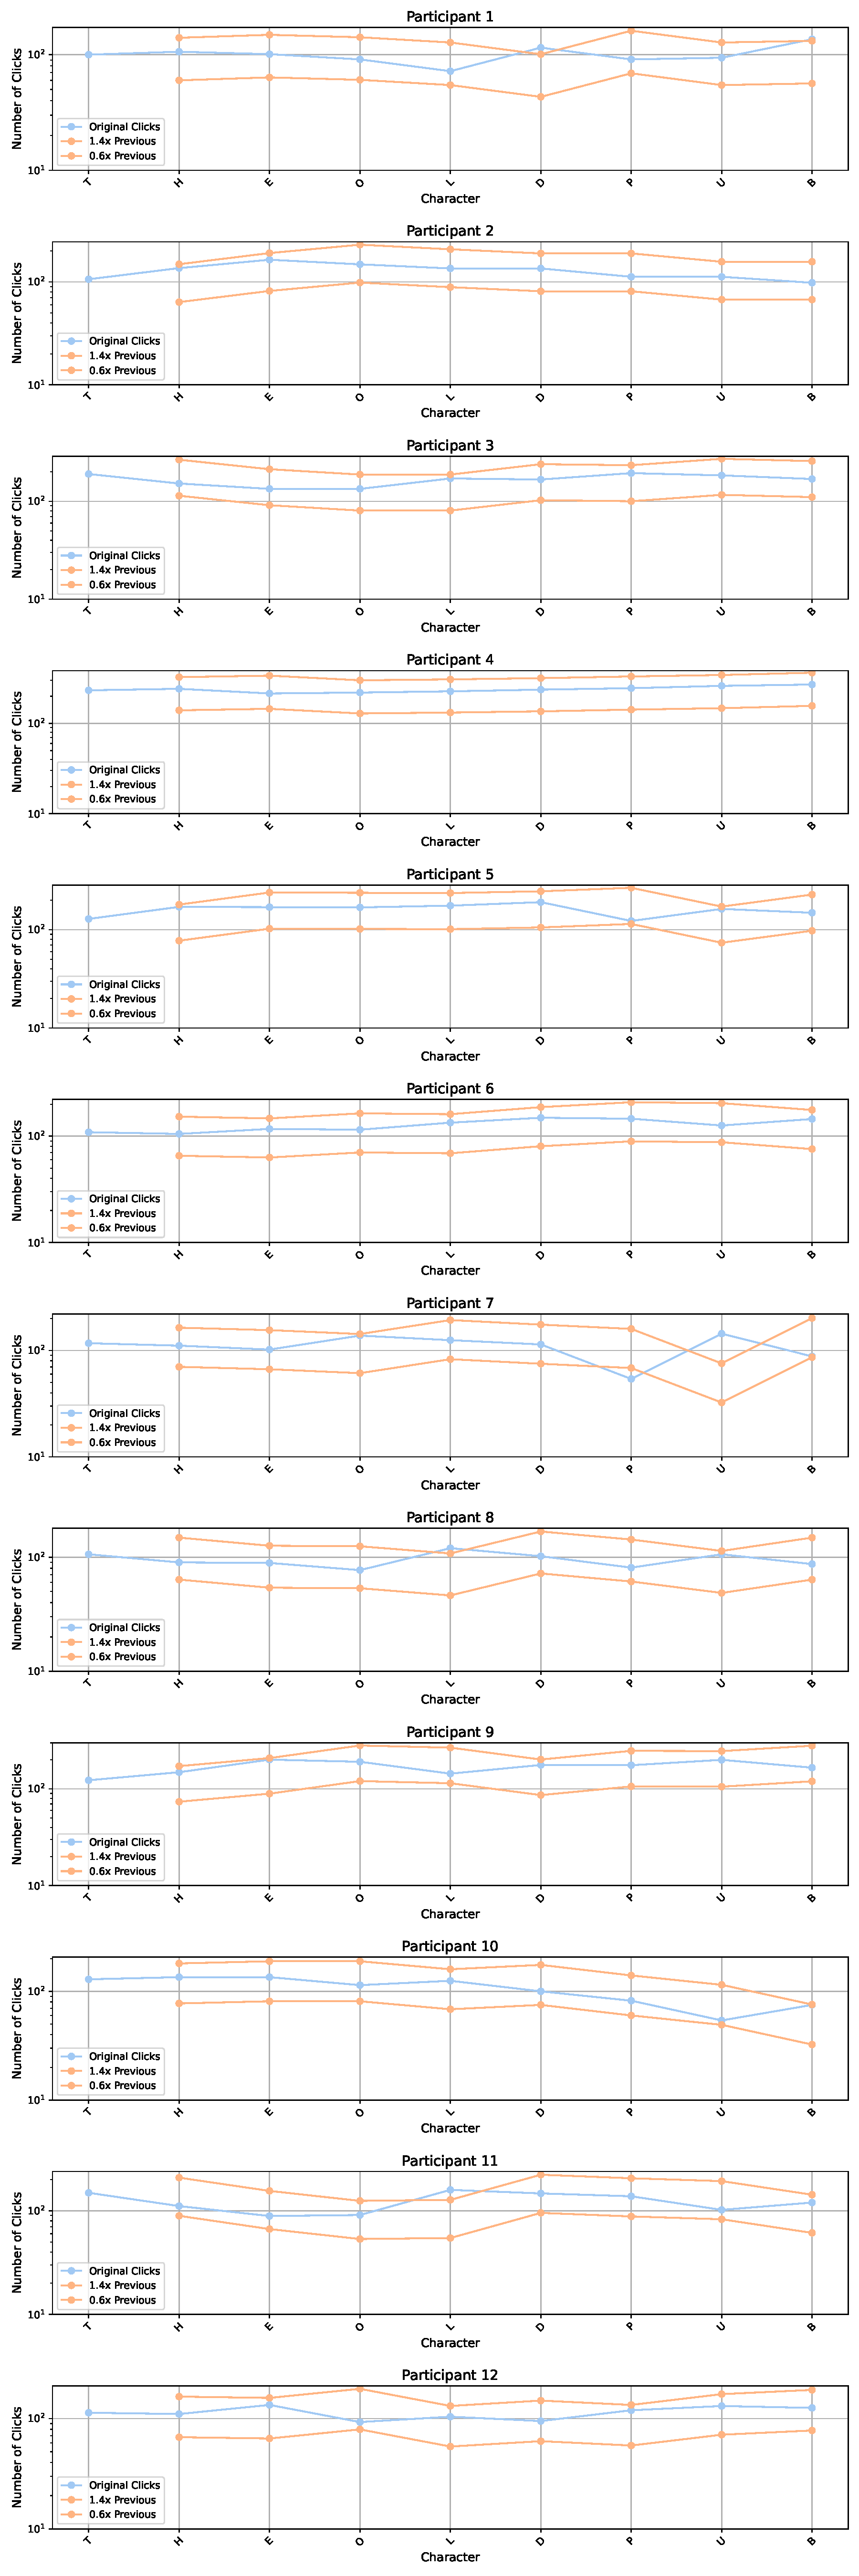
\includegraphics[width=0.5\linewidth]{src/pictures/Study1Data_questionnaire/participantPlots_study1.pdf}
    \caption{Participant click scores.}
    \label{fig:participant_clicks-firstStudy}
\end{figure}

In the first study, we interviewed 12 participants (3 female, 9 male), aged between 22 and 55, with an average age of 28.67 and a median age of 27 years. Of these, 11 were right-handed, and one was left-handed, as shown in \autoref{tab:study1_participant_data}. None of the participants had prior knowledge of Braille.

First, we assessed the validity of our data by ensuring that the participants were focused on the game and not on the sensations themselves. To do so, we measured the click rate for each character to detect any differences in performance. Given that participants tended to become more fatigued later in the game, we compared the click rates with those from the previous round to determine whether the data showed a 40\% improvement or decline, as indicated by the two red lines in \autoref{fig:participant_clicks-firstStudy}. As shown, the data passed the test, with the exception of participant 7, where the observed difference can be attributed to the stimulus change and the completion of questionnaires between sessions.

\subsubsection{First study experiment results}

\begin{figure}
    \centering
    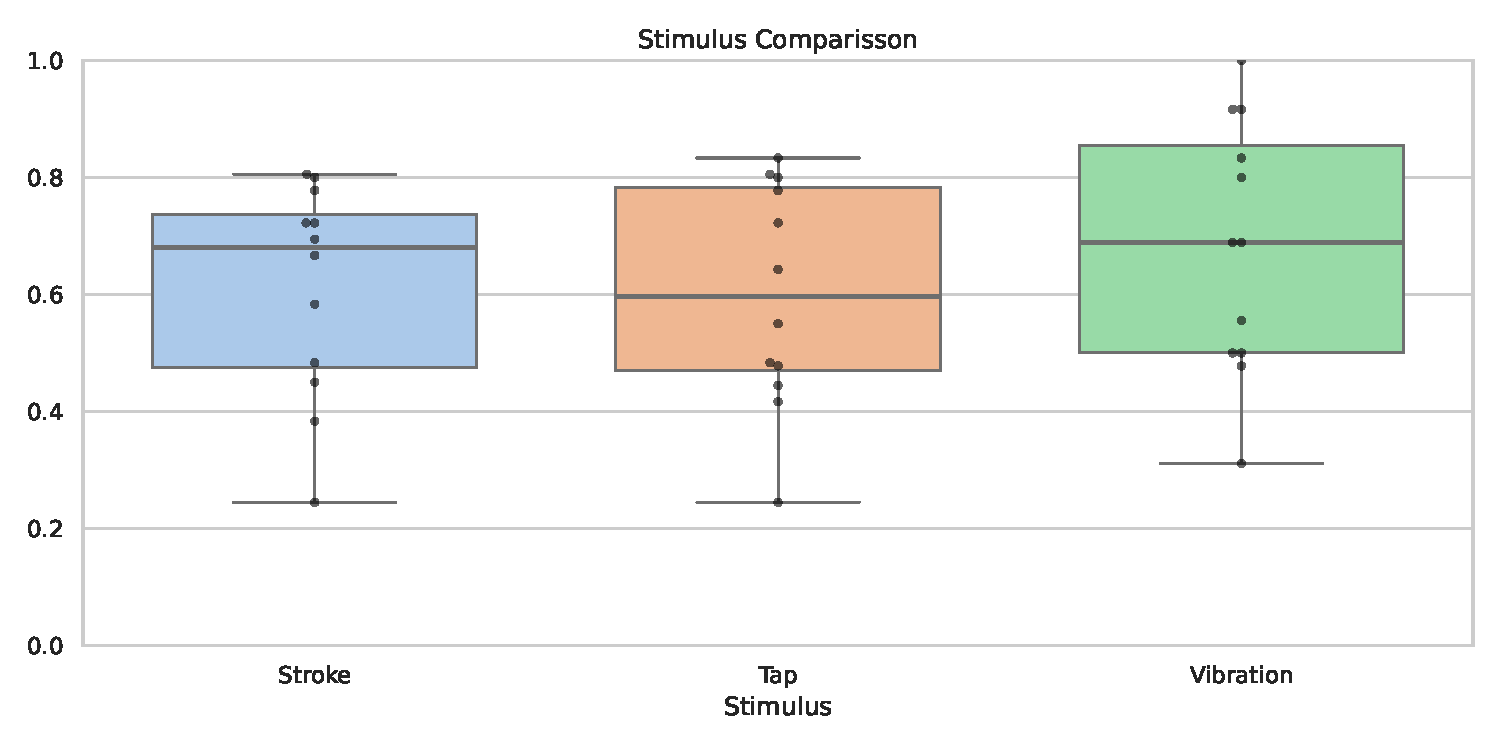
\includegraphics[width=0.5\linewidth]{src/pictures/Study1Data_Experiment/learn_data_averaged.pdf}
    \caption{Character-test results during learning for the different stimuli.}
    \label{fig:learning_results}
\end{figure}
% The \autoref{fig:learning_results} depict the results we measured the averaged values for each stimuli after the learning of each character.
% As can be seen, the medians are rather similar with values of
% about $0.7$ for stroke, $0.6$ for Tap and $0.7$ for Vilolation.
% Both Stroke, and Tap look rather similar, however, the Tap boxplot is different, as its's lowest value is higher thanthe lowest value for the other two.
% Moreover it is the only one, where one participant reached a perfect score.

% Testing the significance with a resulted in a non-significance with a friedman test with a test statistic of $2.4255$ p-value of $0.2974$ as depicted in \autoref{table:learning_results_firstStudy}

The \autoref{fig:learning_results} shows the averaged results for each stimulus after participants completed the learning phase for each character.

The median scores are relatively similar: approximately $0.7$ for Stroke, $0.6$ for Tap, and $0.7$ for Violation. While Stroke and Tap appear similar overall, the Tap boxplot differs in that its minimum value is higher than those of the other two stimuli. Notably, Tap is also the only condition in which a participant achieved a perfect score.

To test for statistical significance, we conducted a Friedman test. The results were not significant, with a test statistic of $2.4255$ and a $p$-value of $0.2974$, as shown in \autoref{table:learning_results_firstStudy}.


\begin{table}[ht]
\resizebox{\columnwidth}{!}{
\centering
\begin{tabular}{|l|l|l|l|l|}
\hline
\textbf{Question}                              & \textbf{Friedman test statistic}& \textbf{p-value}       & \textbf{Significance}           &\textbf{Kendall's W}\\ \hline
Learning Data& 2.4255& 0.2974& Not Significant                 &0.1011\\\hline
\end{tabular}}
\caption{Results of the Friedman significance tests during learning with a Kendall's W Effect Size.}
\label{table:learning_results_firstStudy}
\end{table}

\begin{figure}
    \centering
    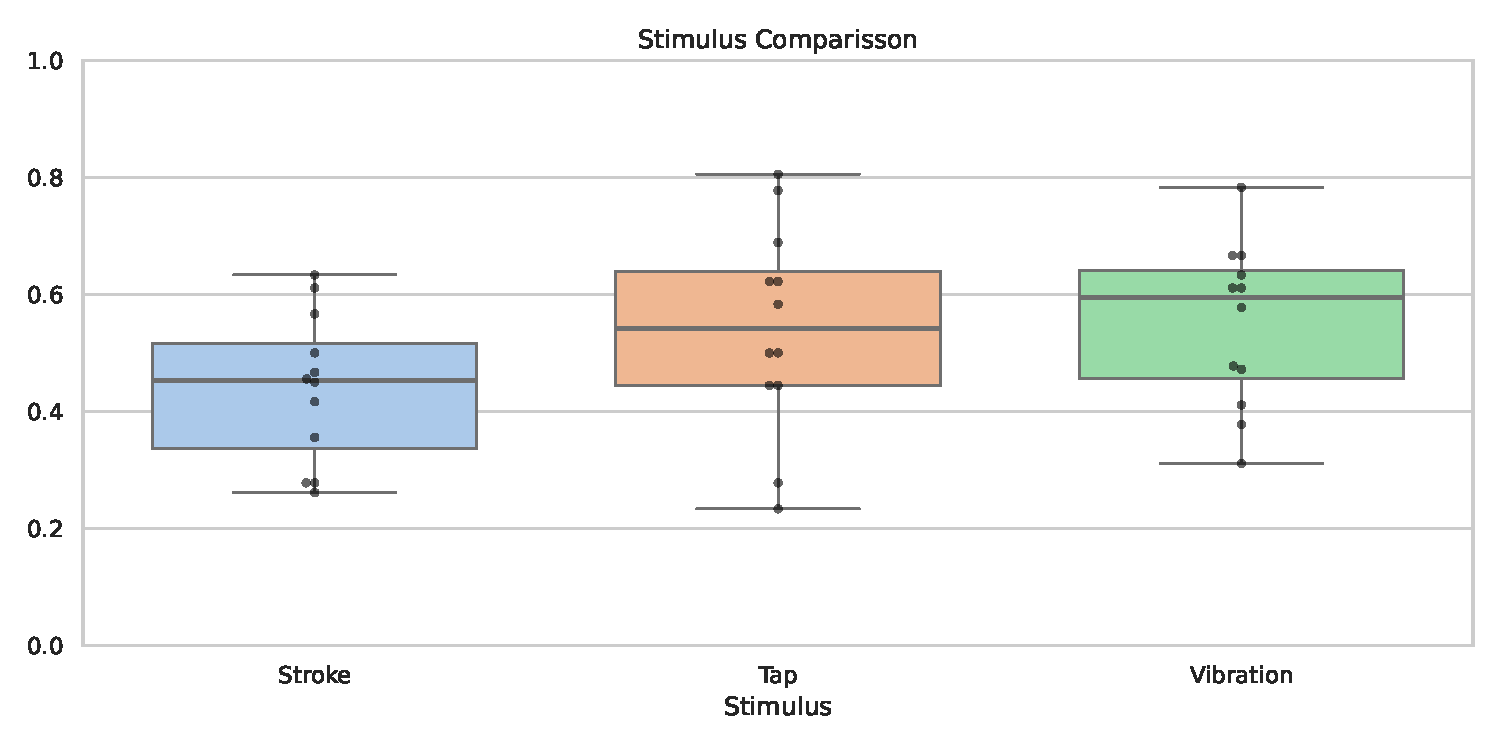
\includegraphics[width=0.5\linewidth]{src/pictures/Study1Data_Experiment/test_data_averaged.pdf}
    \caption{Word-test results for the different stimuli.}
    \label{fig:testing_results}
\end{figure}
% After all the learning was completed, we condicted the whole word tests.
% The averaged word test resukts are depicted in \autoref{fig:testing_results}.
% As can be seen, the strokeing results are slightly worse than the tapping and vibration one, where the bpxplots look rather similar.
% However, it can be seen, that the median is the best for the vibraiton stimili with a median of $0.59$ vs $0.525$ for tapping and $0.45$ for stroking.

% Testing for a significant difference between the stimuli fith a friedman test resulted in a test statistic of 3.5 an a p value of 0.1738 showing no significant difference as depicted in \autoref{table:testing_results_firstStudy}.
After completing all learning phases, we conducted the whole word tests. The averaged results are shown in \autoref{fig:testing_results}.

Overall, the Stroking condition performed slightly worse than Tapping and Vibration, whose boxplots appear similar. Among the three, the Vibration stimulus yielded the highest median accuracy at $0.59$, followed by Tapping at $0.525$ and Stroking at $0.45$.

To assess statistical significance, we performed a Friedman test. The result was not significant, with a test statistic of $3.5$ and a $p$-value of $0.1738$, as shown in \autoref{table:testing_results_firstStudy}.


\begin{table}[ht]
\resizebox{\columnwidth}{!}{
\centering
\begin{tabular}{|l|l|l|l|l|}
\hline
\textbf{Question}                              & \textbf{Friedman test statistic}& \textbf{p-value}       & \textbf{Significance}           &Kendall's W\\ \hline
Testing Data& 3.5& 0.1738& Not Significant                 &0.1458\\\hline
\end{tabular}}
\caption{Results of the Friedman significance tests during learning with a Kendall's W Effect Size.}
\label{table:testing_results_firstStudy}
\end{table}


\subsubsection{First study Questionnaire results}


\begin{figure}
    \centering
    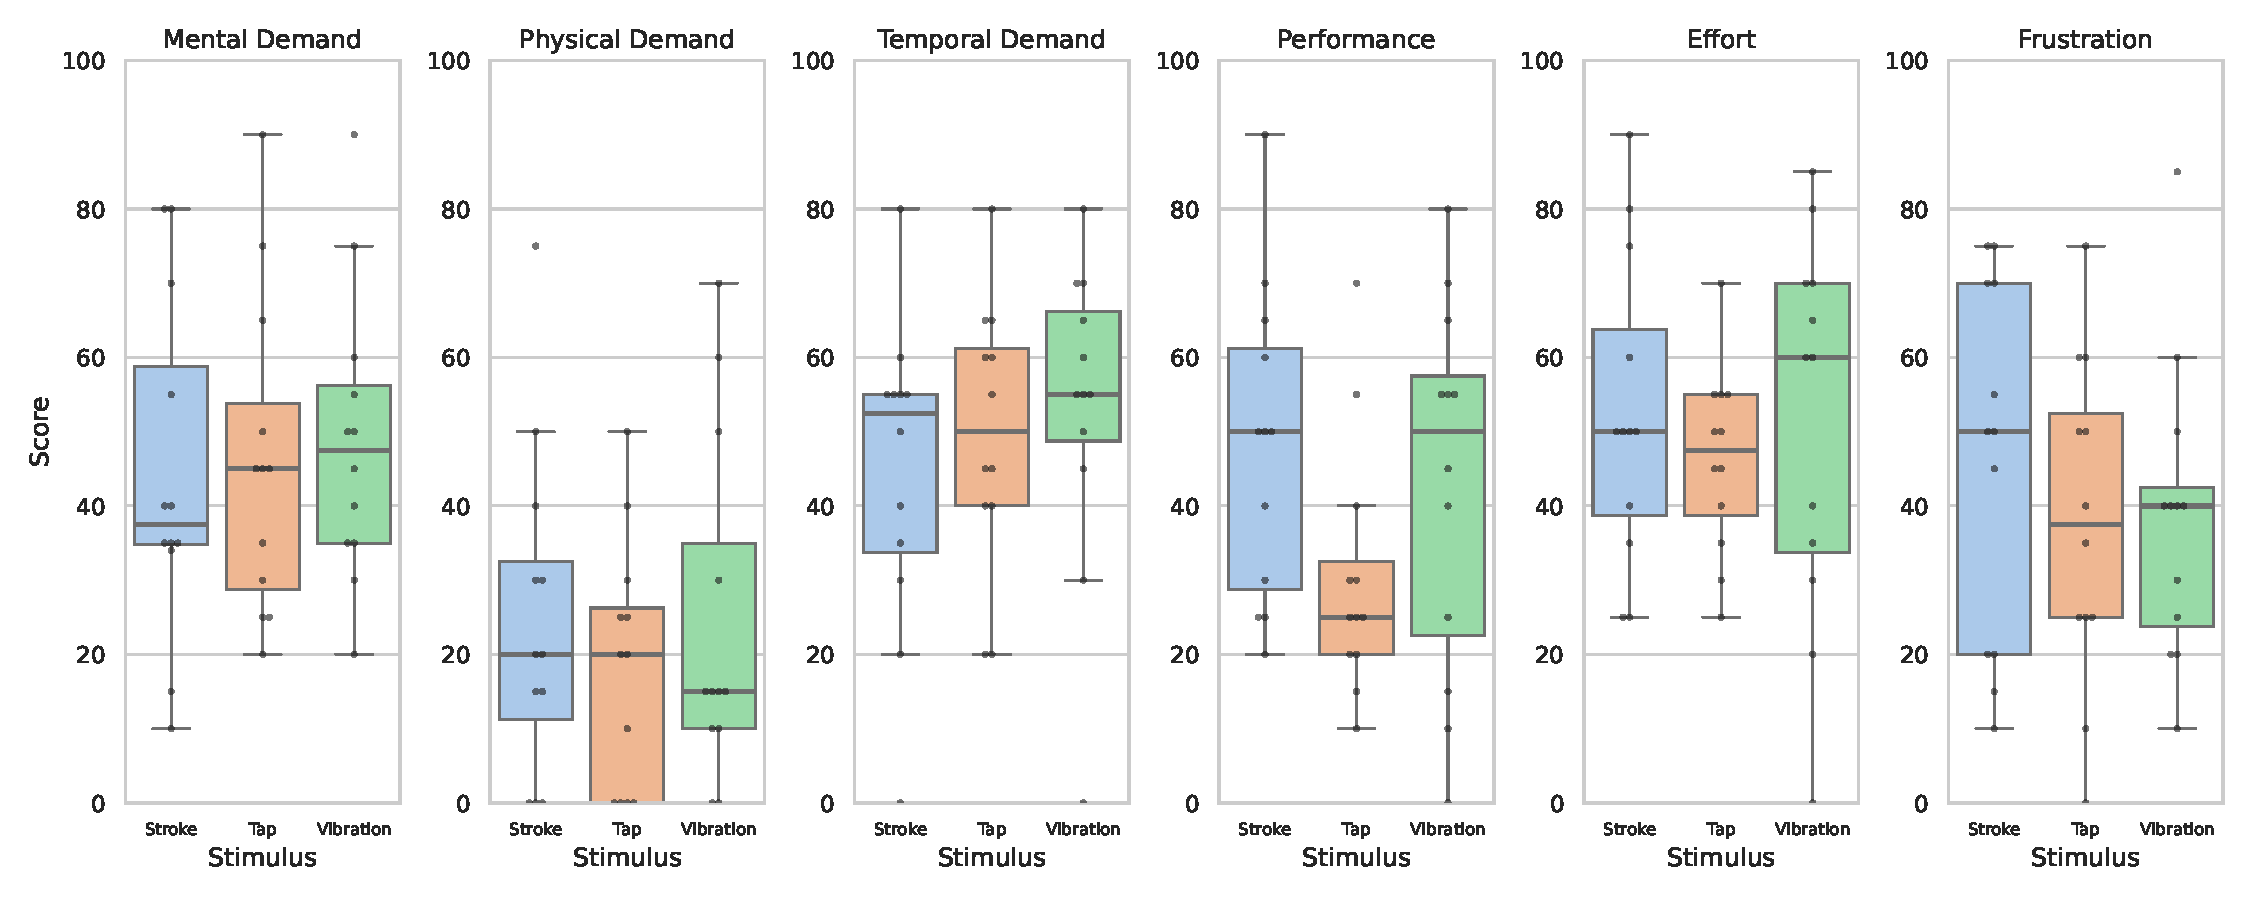
\includegraphics[width=0.5\linewidth]{src/pictures/Study1Data_questionnaire/NasaTLX_study1.pdf}
    \caption{Nasa TLX results for the first study.}
    \label{fig:nasa_tlx_first_study}
\end{figure}
% After each study was conducted, we measuered the nasa tlx resulted as depicted in \autoref{fig:nasa_tlx_first_study}.

% The largest differences can be seen in the performance chategory, where the tapping results were worse than the stroke and vibration ones as depicted with the medians of about 50 for the stroke and vibration compared to the 25 for tapping.
% Another larger difference can be seen for the median in the dimension Frustration and effort.
% With medians of about 50, 37.5 and 40 for stroking tapping and vibration respectively in the frustration category.
% And medians of about 50, 47.5 and 60 for the stroking, tapping and vibration respectively in the effort category.

% However, after checking for the significance, we only found a significance in the performance dimension with an friedman statistic of $7.0870$ with an p-value of $0.0289$ and an Kendall's W effect size of $0.2953$ as depicted in \autoref{table:nasaTLX_significance_firstStudy_nonParam}.

% After conducting a post-hock test, that is depicted in \autoref{table:nasaTLX_significance_firstStudy_nonParam_PostHock}, we showed, that the approaching signifficance is between tapping and stroking with an wilcoxon test statistic of $2.0$ and an p-value of $0.0057$.

% However, after correcting the alpha with a Bonferroni-corrected alpha of $0.0167$, we only see, that the signifficance is approaching signifficant.

After each study, we measured the NASA-TLX scores, as shown in \autoref{fig:nasa_tlx_first_study}.

The most noticeable differences appeared in the Performance category. Here, Tapping scored worse than both Stroking and Vibration, with median values of approximately $50$ for Stroking and Vibration, compared to $25$ for Tapping. Additional differences were observed in the Frustration and Effort dimensions. In the Frustration category, the median scores were roughly $50$ for Stroking, $37.5$ for Tapping, and $40$ for Vibration. For Effort, the median scores were about $50$, $47.5$, and $60$, respectively.

Significance testing revealed a statistically significant difference only in the Performance dimension, with a Friedman test statistic of $7.0870$, a $p$-value of $0.0289$, and a Kendall’s W effect size of $0.2953$ (\autoref{table:nasaTLX_significance_firstStudy_nonParam}).

A follow-up post-hoc analysis, shown in \autoref{table:nasaTLX_significance_firstStudy_nonParam_PostHock}, indicated that the potential source of this difference lies between the Tapping and Stroking conditions. A Wilcoxon signed-rank test yielded a test statistic of $2.0$ and a $p$-value of $0.0057$.

However, after applying a Bonferroni correction with an adjusted alpha level of $0.0167$, this difference is considered to be approaching significance, but not statistically significant.



\begin{table}[ht]
\resizebox{\columnwidth}{!}{
\centering
\begin{tabular}{|l|l|l|l|l|}
\hline
\textbf{Question}        & \textbf{Friedman statistic}& \textbf{p-value}       & \textbf{Significance}           &\textbf{Kendall's W Effect Size}\\ \hline
\textbf{Mental Demand}    & 0.0476& 0.9765& Not Significant                 &0.002\\ \hline
\textbf{Physical Demand}  & 0.4375& 0.8035& Not Significant                 &0.0182\\ \hline
\textbf{Temporal Demand}  & 4.2273& 0.1208& Not Significant                 &0.1761\\ \hline
\textbf{Performance}      & 7.0870& 0.0289& \textbf{Significant}&0.2953\\ \hline
\textbf{Effort}           & 1.5652& 0.4572& Not Significant                 &0.0652\\ \hline
\textbf{Frustration}      & 2.2609& 0.3229& Not Significant                 &0.0942\\ \hline
\end{tabular}}
\caption{Results of the Friedman significance tests for the different NasaTLX dimensions with a Kendall's W Effect Size.}
\label{table:nasaTLX_significance_firstStudy_nonParam}
\end{table}


\begin{table}[ht]
\resizebox{\columnwidth}{!}{
\centering
\begin{tabular}{|l|l|l|l|l|}
\hline
\textbf{Question}        & \textbf{Difference}& \textbf{Wilcoxon w- statistic}& \textbf{p-value}       &\textbf{Significance}           \\ \hline
\textbf{Performance} (POST-HOCK)& T vs S& 2.0& 0.0057&approaching \textbf{Significant}\\ \hline
& T vs V& 15.5& 0.1188&Not Significant                 \\ \hline
& S vs V& 30.0& 0.5186&Not Significant                 \\\hline
\end{tabular}}
\caption{Results of the Posthock Analyse for the NasaTLX performance dimension with a Wilcoxon test.}
\label{table:nasaTLX_significance_firstStudy_nonParam_PostHock}
\end{table}



\begin{figure}
    \centering
    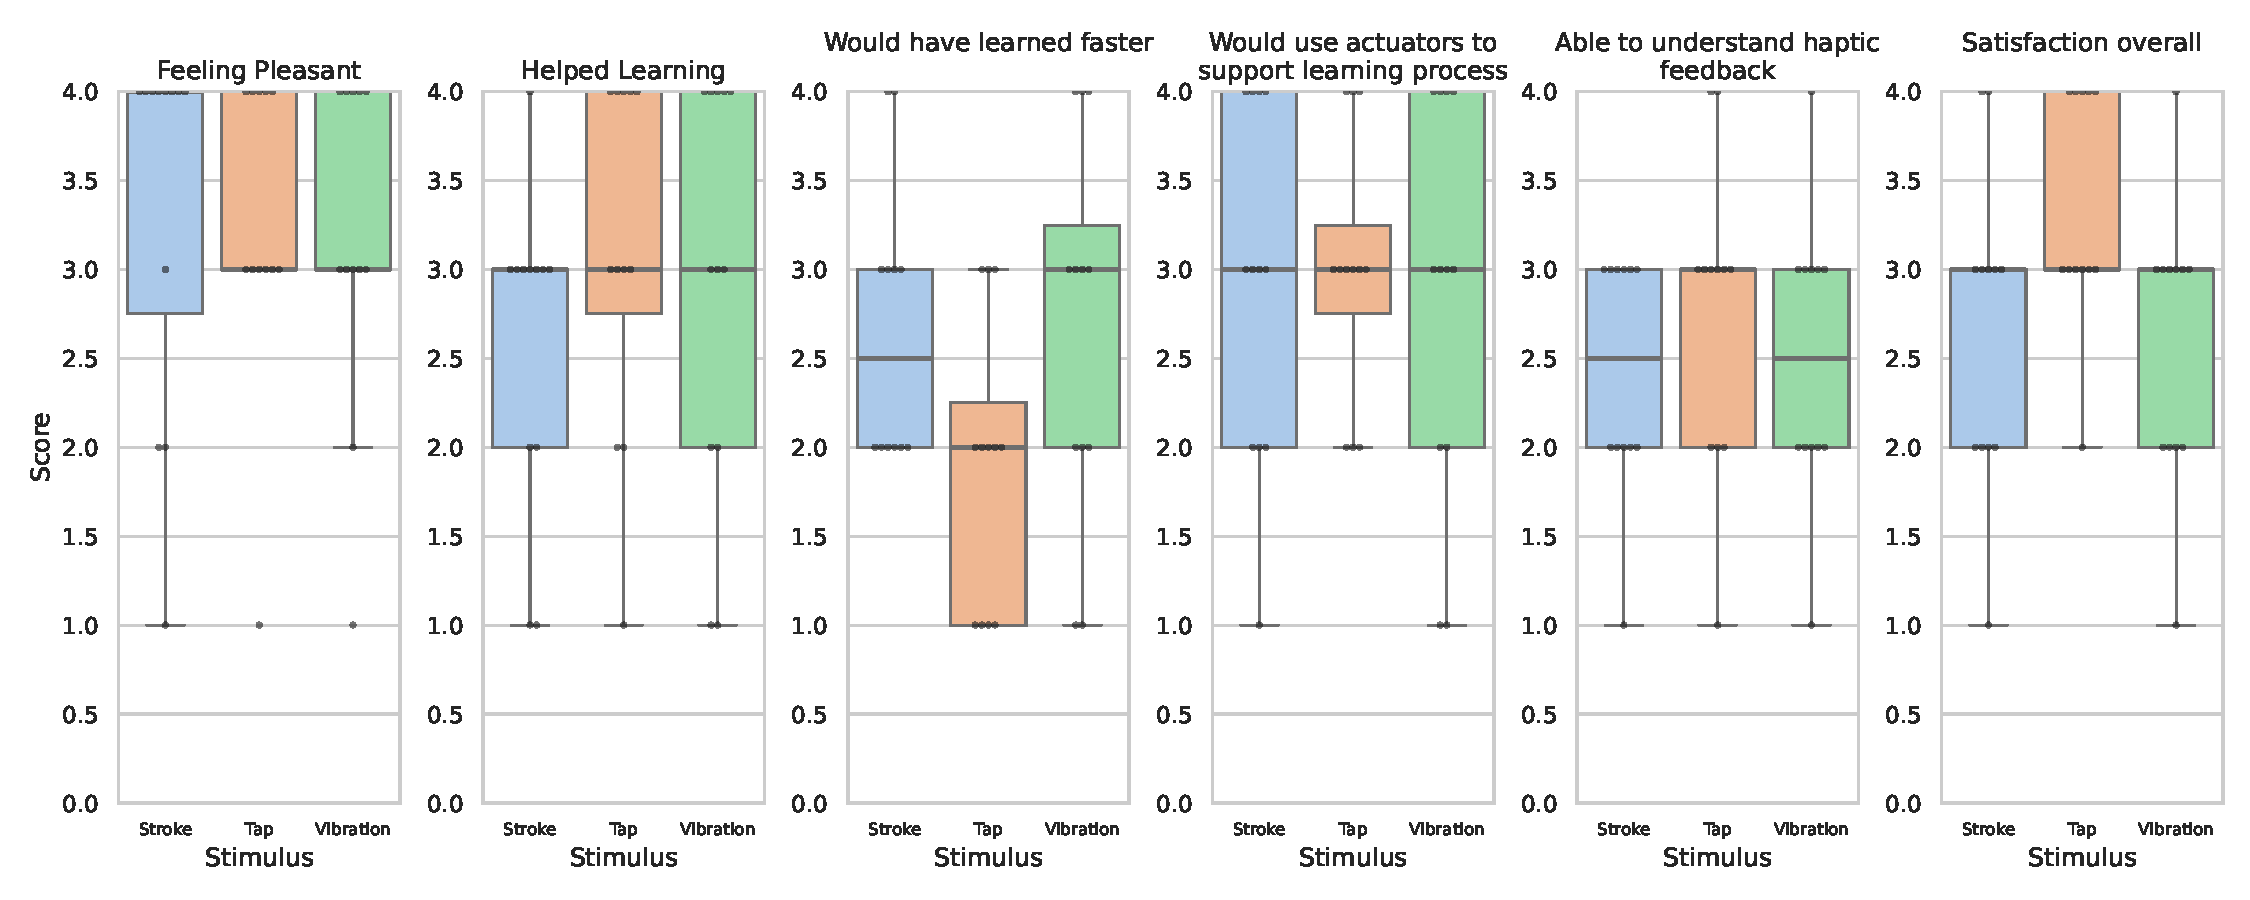
\includegraphics[width=0.5\linewidth]{src/pictures/Study1Data_questionnaire/questions_special_study1.pdf}
    \caption{Usability questions results for the first study.}
    \label{fig:special_study_first_study}
\end{figure}
% After learning a word with a stimuli, we also tested for the usability for six dimensions, whose results are depicted in \autoref{fig:special_study_first_study} 

% Larger differences can be seen in the medians for \enquote{Feeling Pleasant} with medians of 3.0 for tapping and viobration and 4.0 for stroking.

% another larger difference can be seen in the medians in the \enquote{able to understand hapric feedback} dimension with medians of 2.5 for vibration and stroking and 3 for tapping, however the boxplots are basically the same with outliers also being similar except fort the stroking condition, which didn't have anyone voting for a perfect score.

% Another larger differecne can be seen in the dimension \enquote{satisfaction overall}, for which the tapping stimulus is the best one, as the quantile range is between 3 and 4 for tapping and 2 and 3 for stroking and vibration.

% other larger differences can be seen in the category \enquote{helped learning}, where the medians are the same at 3, but their q1-q3 quantile differences are 2-3 for stroke, 2.75-4 for tapping and 2-4 for vibration.

% moreover another notewirthy difference is at \enquote{would have learned faster}, with medians of 2.5 for vibration, 2 for tapping and 3 for stroking and with q1-q3 differences of 2-3 for strking, 1-2.25 to tapping and 2-3.25 for vibration.

% We conducted Friedman signifficance tests given this data, whose results are plotted here \autoref{table:individualQuestions_significance_firstStudy}.
% As can be see, the dimensions \enquote{Helped Learning}, \enquote{Would have learned faster} and \enquote{satisfaction overall} are statistical signifficant with p-values of 0.0701 for \enquote{helped learning}, 0.0104 for \enquote{Would have learned faster} and 0.0027 for \enquote{Satisfaction overall}.

% Afterwards, we did the post hock analysis for those dimensions, as can be shown in \autoref{table:selfAssessment_significance_firstStudy_nonParam_PostHock}.
% For the dimension \enquote{Helped Learning} the posthock didn't show anything,
% For the dimension \enquote{Would have learned faster} there is a difference between T and S with a p-value of $0.0027$ that shows a signifficance.
% For the dimension of \enquote{Satisfaction overall}, there are signifficant differences between T vs S and T vs V with p-values of $0.0114$ and $0.0139$.

% Using the Bonferroni-corrected alpha, we show, that the \enquote{helped learning} with $0.0167$ show that the dimension with $0.0701$ is not signifficant.
% The dimension \enquote{would have learned faster} has a Bonferroni-corrected alpha of $0.0167$ is still signifficant with $0.0104$.
% And the dimension \enquote{Satisfaction overall} with a p-value of $0.0027$ is after the Bonferroni-corrected alpha of $ 0.0167$ is according to that not signifficant.
After learning a word using each stimulus, we evaluated usability across six dimensions. The results are shown in \autoref{fig:special_study_first_study}.

Notable differences emerged in the \enquote{Feeling Pleasant} dimension, with median ratings of $4.0$ for Stroking and $3.0$ for both Tapping and Vibration. Another difference was observed in \enquote{Able to understand haptic feedback}, where medians were $2.5$ for Vibration and Stroking, and $3.0$ for Tapping. However, the boxplots were nearly identical across all conditions, with similar outliers—except for Stroking, which had no participants selecting the highest rating.

In the \enquote{Satisfaction Overall} dimension, Tapping showed the highest ratings, with an interquartile range (IQR) from $3$ to $4$, compared to an IQR of $2$ to $3$ for both Stroking and Vibration. Additional variation appeared in \enquote{Helped Learning}; although all stimuli had the same median of $3.0$, their IQRs differed: $2$–$3$ for Stroking, $2.75$–$4$ for Tapping, and $2$–$4$ for Vibration. 

A further difference was seen in the \enquote{Would have learned faster} dimension, where Stroking had a median of $3.0$, Vibration $2.5$, and Tapping $2.0$. The IQRs were $2$–$3$ for Stroking, $2$–$3.25$ for Vibration, and $1$–$2.25$ for Tapping.

We performed Friedman tests to assess statistical significance, with results shown in \autoref{table:individualQuestions_significance_firstStudy}. Statistically significant effects were found in the dimensions \enquote{Would have learned faster} ($p = 0.0104$) and \enquote{Satisfaction Overall} ($p = 0.0027$), while \enquote{Helped Learning} showed a trend toward significance with a $p$-value of $0.0701$.

Post-hoc Wilcoxon tests, presented in \autoref{table:selfAssessment_significance_firstStudy_nonParam_PostHock}, revealed no significant pairwise differences for \enquote{Helped Learning}. For \enquote{Would have learned faster}, a significant difference was found between Tapping and Stroking ($p = 0.0027$). In the case of \enquote{Satisfaction Overall}, significant differences were found between Tapping and Stroking ($p = 0.0114$), as well as between Tapping and Vibration ($p = 0.0139$).

After applying the Bonferroni correction with an adjusted alpha of $0.0167$, \enquote{Helped Learning} was no longer considered significant. However, both \enquote{Would have learned faster} and \enquote{Satisfaction Overall} remained statistically significant under the corrected threshold.


\begin{table}[ht]
\resizebox{\columnwidth}{!}{
\centering
\begin{tabular}{|l|l|l|l|l|}
\hline
\textbf{Question}                              & \textbf{Friedman statistic}& \textbf{p-value}       & \textbf{Significance}           &\textbf{Kendall's W Effect Size}\\ \hline
\textbf{Feeling Pleasant}                      & 0.8276& 0.6611& Not Significant                 &0.0345\\ \hline
\textbf{Helped Learning}                       & 5.3143& 0.0701& approaching
\textbf{Significant}&0.2214\\ \hline
\textbf{Would have learned faster}             & 9.1351& 0.0104& \textbf{Significant}&0.3806\\ \hline
\textbf{Would use actuators to support learning process} & 0.5600& 0.7558& Not Significant                 &0.0233\\ \hline
\textbf{Able to understand haptic feedback}    & 2.5455& 0.2801& Not Significant                 &0.1061\\ \hline
\textbf{Satisfaction overall}& 11.84& 0.0027& \textbf{Significant}&0.4933\\ \hline
\end{tabular}}
\caption{Results of the Kruskal-Wallis significance tests for the different self-assessment dimensions with a $\eta^2$ Effect Size.}
\label{table:individualQuestions_significance_firstStudy}
\end{table}


\begin{table}[ht]
\resizebox{\columnwidth}{!}{
\centering
\begin{tabular}{|l|l|l|l|l|}
\hline
\textbf{Question}        & \textbf{Difference}& \textbf{Wilcoxon w- statistic}& \textbf{p-value}       &\textbf{Significance}           \\ \hline
\textbf{Helped Learning} (POST-HOCK)& T vs S& 7.5& 0.1236&Not Significant                 \\
& T vs V& 5.0& 0.4795&Not Significant                 \\
& S vs V& 21.0& 0.2558&Not Significant                 \\\hline
 \textbf{Would have learned faster} (POST-HOCK)& T vs S& 0.0& 0.0027&\textbf{Significant}\\
 & T vs V& 11.0& 0.0841&Not Significant                 \\
 & S vs V& 13.5& 0.9309&Not Significant                 \\\hline
 \textbf{Satisfaction overall} (POST-HOCK)& T vs S& 0.0& 0.0114&\textbf{Significant}\\
 & T vs V& 0.0& 0.0139&\textbf{Significant}\\
 & S vs V& 2.0& 0.5637&Not Significant                 \\\hline
\end{tabular}}
\caption{Results of the Posthock Analyse for the self-assessment with a Wilcoxon test.}
\label{table:selfAssessment_significance_firstStudy_nonParam_PostHock}
\end{table}



\begin{figure}
    \centering
    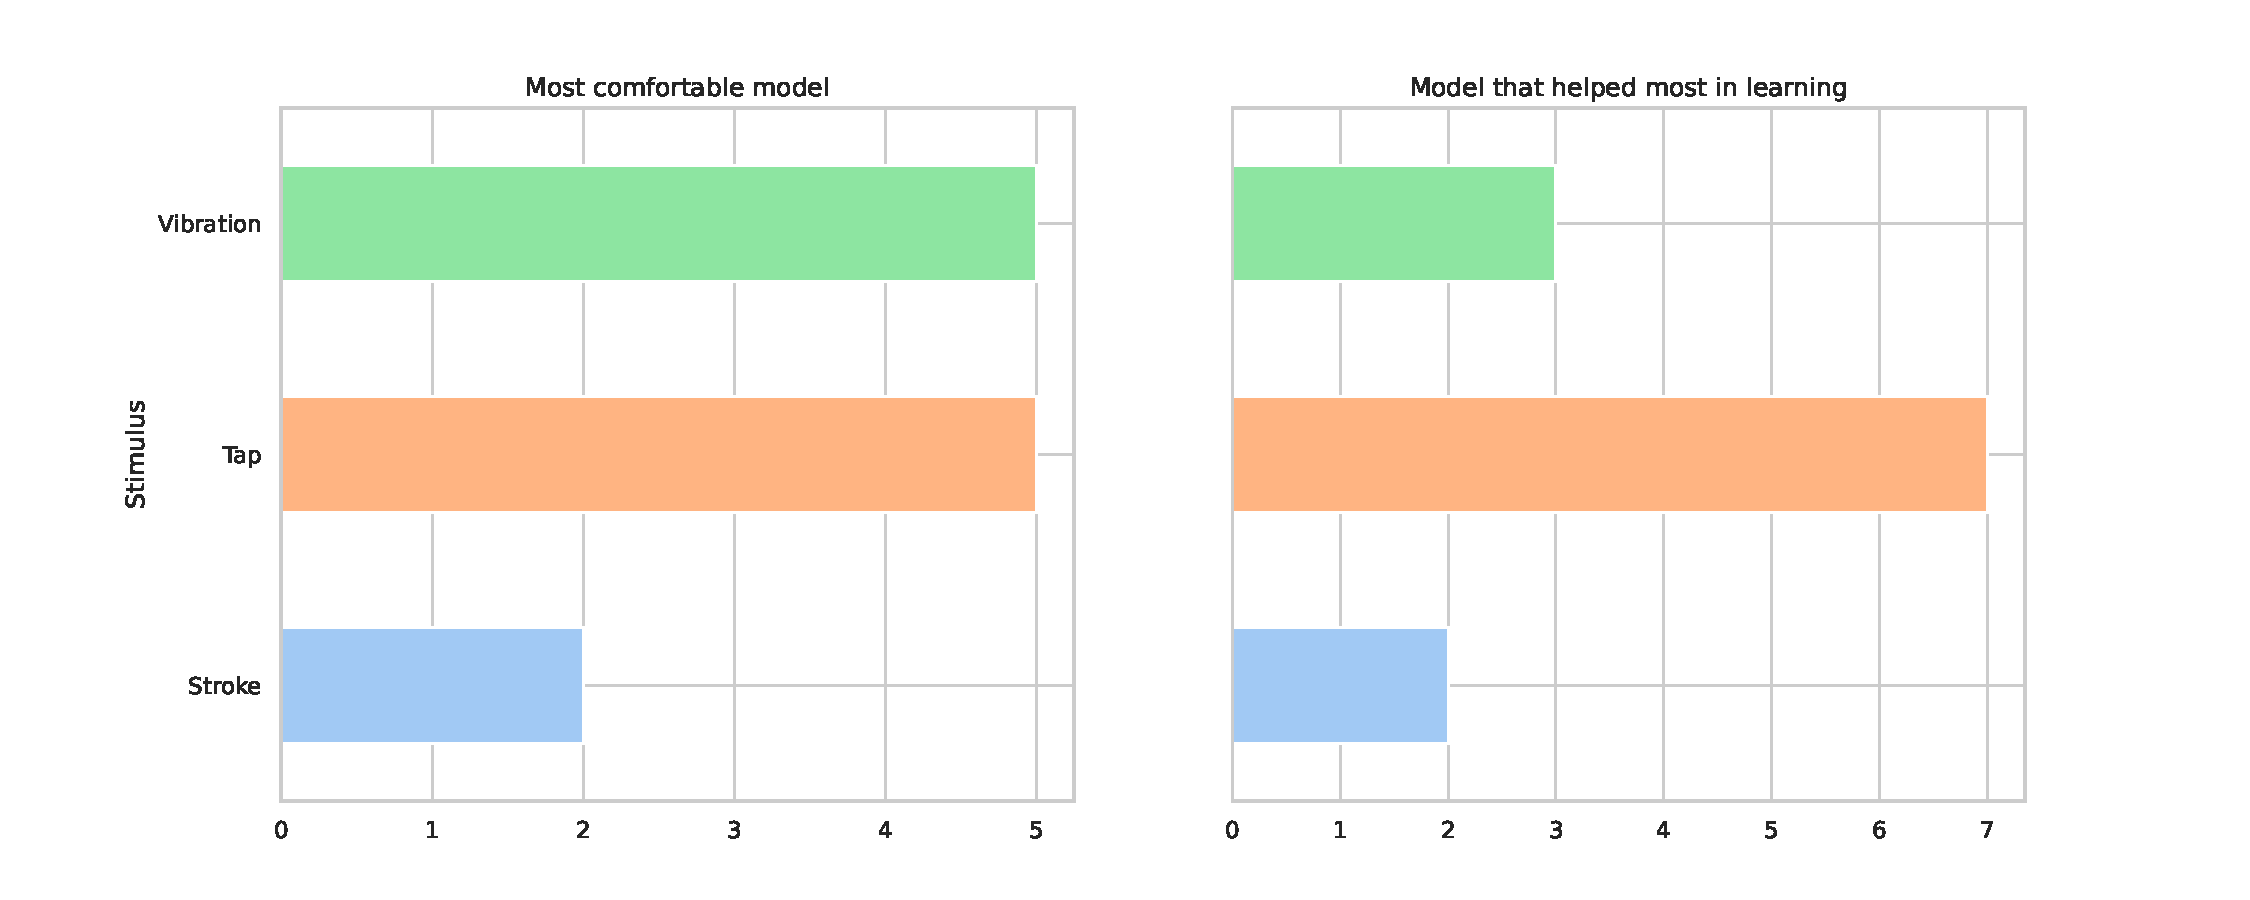
\includegraphics[width=0.5\linewidth]{src/pictures/Study1Data_questionnaire/questions_compare_study1.pdf}
    \caption{Direct Stimuli comparison results.}
    \label{fig:compare_results_first_study}
\end{figure}
% Lastly we compared the different stimuli with each other as depicted in \autoref{fig:compare_results_first_study}.
% Their results show, that the vibration and tapping was the best in the category of \enquote{Most comfortable model} with 5/12 followed by the stroking one with 2/12 and for the category \enquote{Model that helped most in learning} we observed the most participants voting for tapping with 7/12, followed by vibration with 3/12 followed with 2/12.
Lastly, we compared the different stimuli directly, as shown in \autoref{fig:compare_results_first_study}. 

In the category \enquote{Most comfortable model}, both Vibration and Tapping were rated highest, each receiving votes from 5 out of 12 participants. Stroking followed, with 2 out of 12 votes. For the category \enquote{Model that helped most in learning}, Tapping was rated most effective, receiving 7 out of 12 votes, followed by Vibration with 3 votes and Stroking with 2.




\subsection{Second Study}

\begin{table}
\resizebox{\columnwidth}{!}{
    \centering
    \begin{tabular}{|c|c|c|c|} \hline 
        \textbf{Gender}& \textbf{Age}& \textbf{Dominant Hand}& \textbf{Previous Braille Knowledge}\\ \hline 
        F & 21 & R & No\\ \hline 
        M & 61 & L & No\\ \hline 
        M & 23 & R & No\\ \hline 
        F & 27 & R & No\\ \hline 
        F & 29 & R & No\\ \hline 
        M & 23 & R & No\\ \hline 
        M & 26 & R & No\\ \hline 
        M & 23 & R & No\\ \hline
    \end{tabular}}
    \caption{Second study participant data}
    \label{tab:study2_participant_data}
\end{table}
\begin{figure}
    \centering
    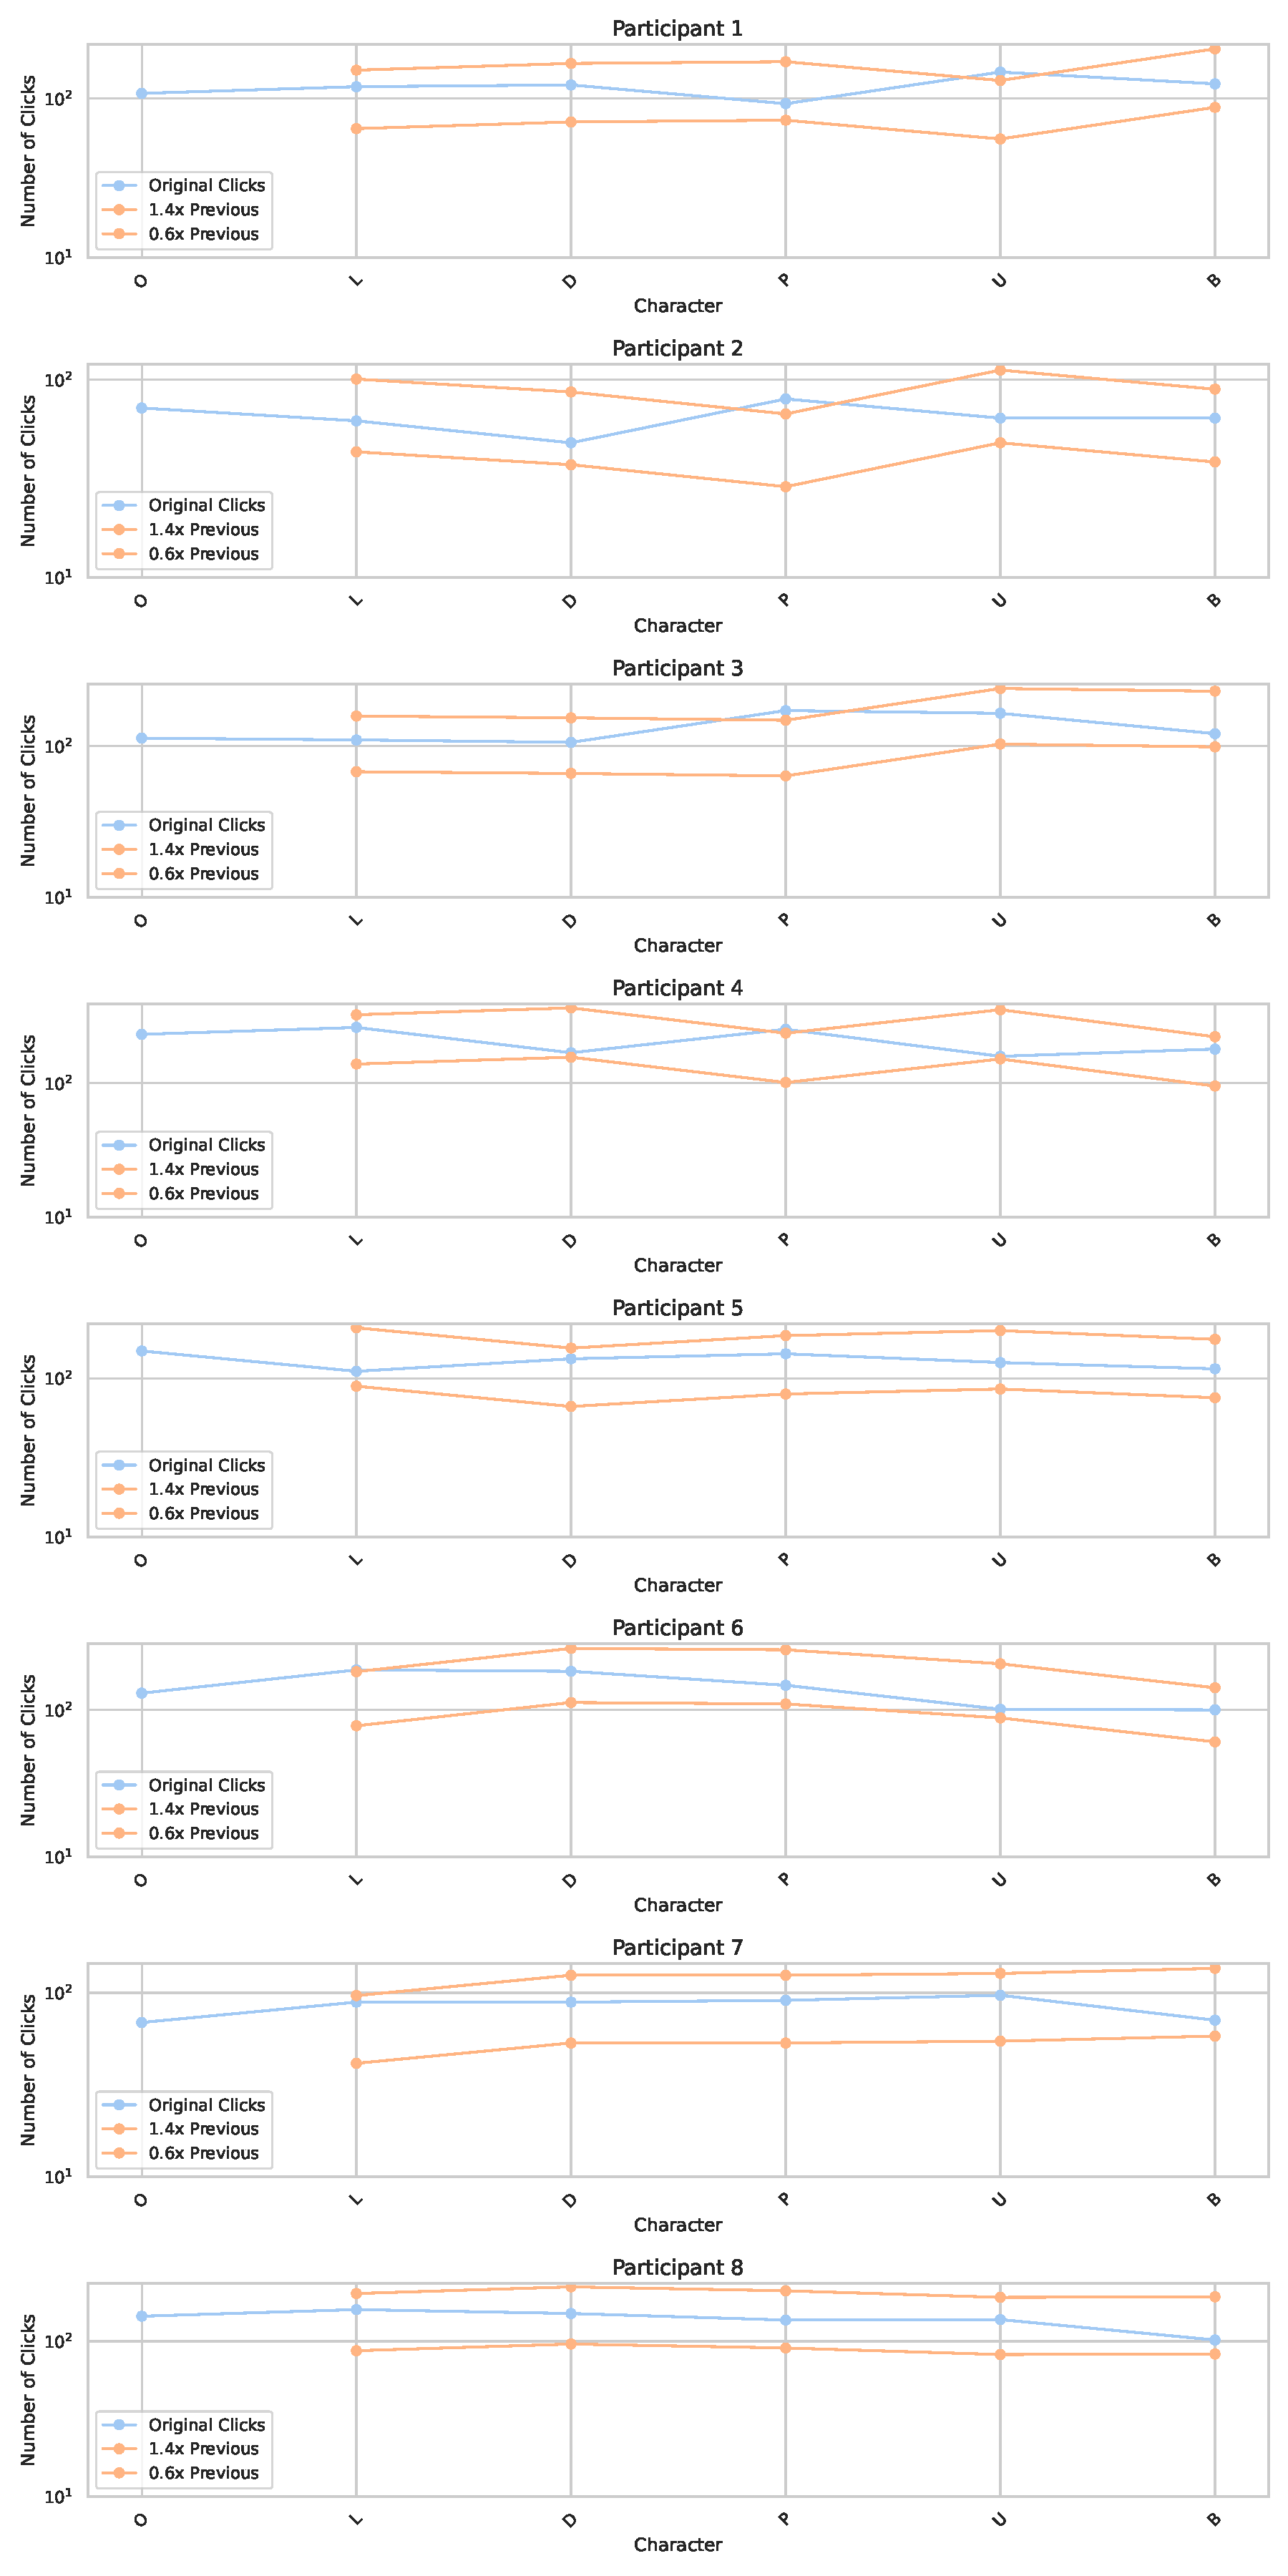
\includegraphics[width=0.5\linewidth]{src/pictures/Study2Data_questionnaire/participantPlots.pdf}
    \caption{Participant click scores.}
    \label{fig:participant_clicks-secondStudy}
\end{figure}

% For the second study, we interviewed 8 participants (5 male, 3 female) aged between 4 and 61 years, with an average age of 29.125 years and a median age of 24.5 years. Of these, 7 participants were right-handed and 1 was left-handed, as shown in \autoref{tab:study2_participant_data}. None of the participants had prior knowledge of Braille.

% As for the first study, we tested the participant click rate for each of the stimuli, to see, if they are different and, henceforth, identicating a participant concentrating on the stimuli instead of the game.
% The corresponding graphs are depicted in \autoref{fig:participant_clicks-secondStudy}.
% As can be seen, none of the values was out of the lower bounds indicating that the participants were focussed on the game.

For the second study, we interviewed eight participants (five male, three female) aged between 4 and 61 years, with an average age of 29.13 years and a median age of 24.5 years. Of these participants, seven were right-handed and one was left-handed, as summarized in \autoref{tab:study2_participant_data}. None of the participants had prior knowledge of Braille.

As in the first study, we measured the participants' click rates for each stimulus to determine whether there were differences that might indicate a shift in attention toward the stimuli rather than the game itself. The corresponding results are presented in \autoref{fig:participant_clicks-secondStudy}. As shown, none of the recorded click rates fell below the lower threshold, suggesting that participants remained focused on the game throughout the experiment.


\subsubsection{Second study experiment results}

\begin{figure}
    \centering
    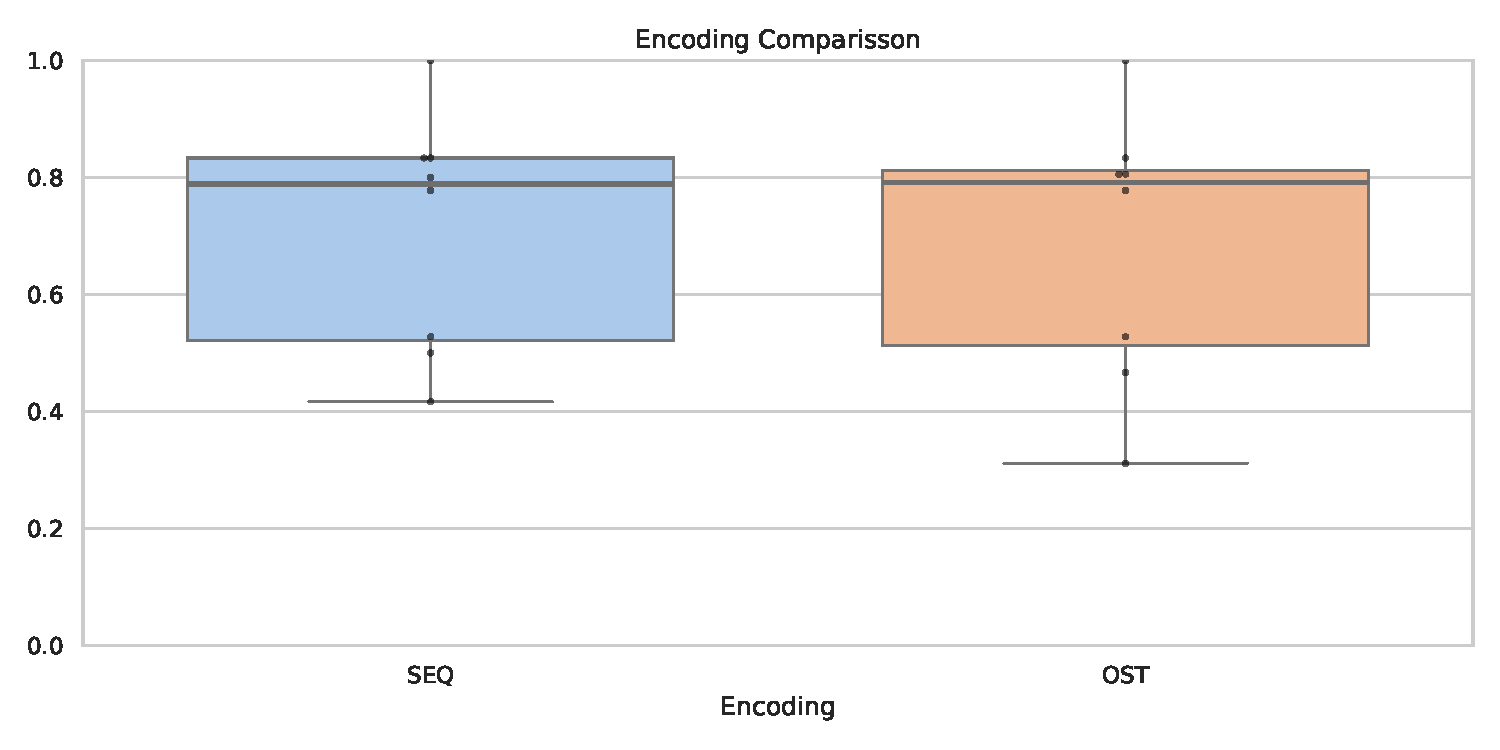
\includegraphics[width=0.5\linewidth]{src/pictures/Study2Data_Experiment/learning_averaged.pdf}
 \caption{Character-test results during learning for the different encodings.}
    \label{fig:learning_results_secondStudy}
\end{figure}
% The \autoref{fig:learning_results_secondStudy} plot shows the difference between the \gls{ost} and \gls{seq} for the learning averaged between the Encodings .
% As can be seen, there is no big difference in the medians with the \gls{ost} median being slightly better with 0.01.

% Moreover, the tests show that there is no significant difference, as can be seen in \autoref{table:learning_results_firstStudy} with an Wilcoxon statistic of 16.0 and p-value of 0.8438.
\autoref{fig:learning_results_secondStudy} illustrates the differences in learning performance between the \gls{ost} and \gls{seq} conditions, averaged across all encodings.

There is no substantial difference between the two, with the \gls{ost} condition showing a slightly higher median by only $0.01$. 

Statistical analysis confirmed that this difference is not significant. As shown in \autoref{table:learning_results_firstStudy}, a Wilcoxon signed-rank test resulted in a test statistic of $16.0$ and a $p$-value of $0.8438$.


\begin{table}[ht]
\resizebox{\columnwidth}{!}{
\centering
\begin{tabular}{|l|l|l|l|l|}
\hline
\textbf{Question}                              & \textbf{Wilcoxon statistic}& \textbf{p-value}       & \textbf{Significance}           &\textbf{Cohens D}\\ \hline
Learning Data& 16.0& 0.8438& Not Significant                 &0.0927\\\hline
\end{tabular}}
\caption{Results of the Wilcoxon significance tests during learning with a Cohens D Effect Size.}
\label{table:learning_results_firstStudy}
\end{table}



\begin{figure}
    \centering
    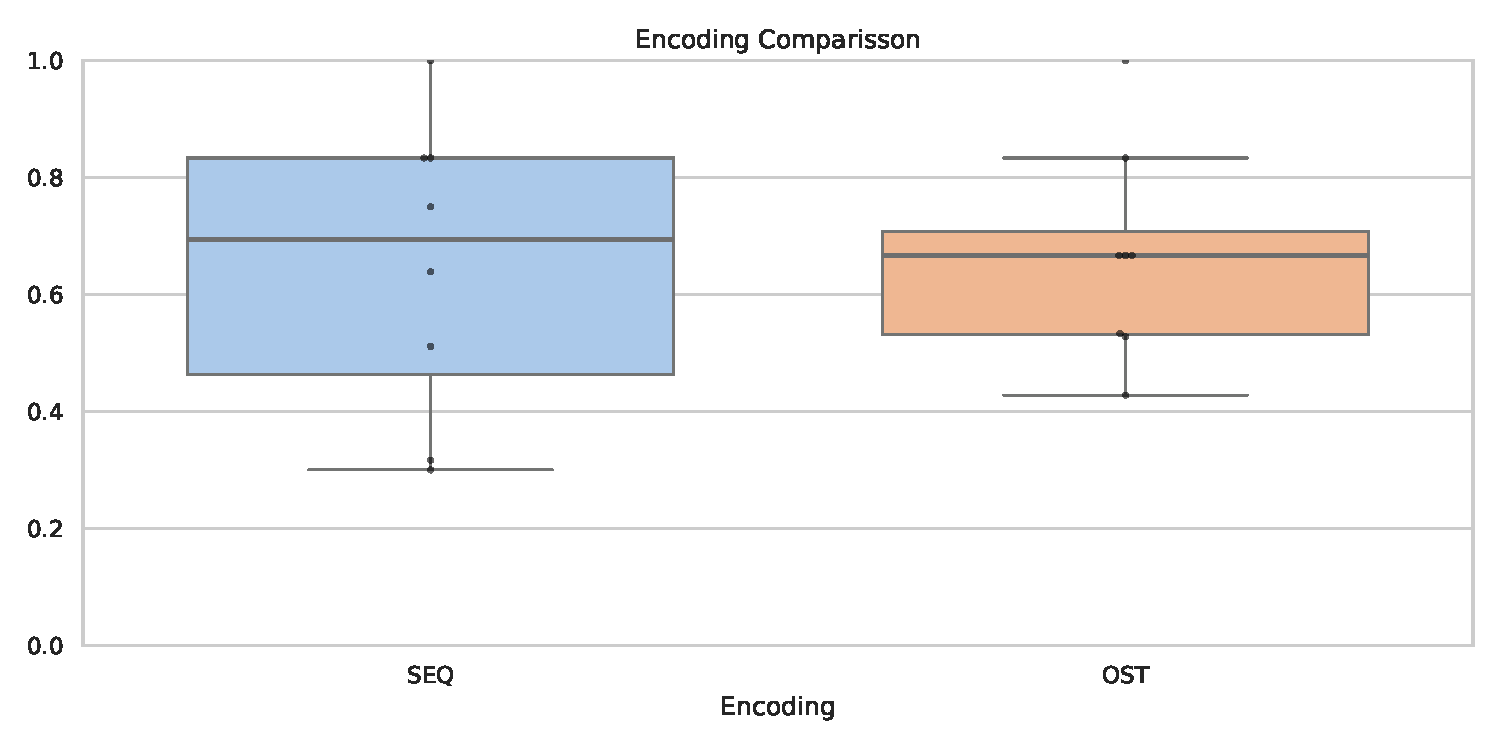
\includegraphics[width=0.5\linewidth]{src/pictures/Study2Data_Experiment/test_averaged-2.pdf}
    \caption{Word-test results for the different encodings.}
    \label{fig:testing_results_secondStudy}
\end{figure}
% After testing the characters with the character test, we plotted their results, shown here \autoref{fig:testing_results_secondStudy}.
% It shows, that there is no big median difference with about 0.7 for \gls{seq} and about 0.675 for \gls{ost},
% however, there can be seen a difference in the Q1-Q3 differences with about 0.425-0.81 for \gls{seq} and 0.51 - 0.7 for \gls{ost}.

% testing for a significance showed, that there is no signifficant difference, as can be seen in \autoref{table:testing_results_firstStudy}, that shows a p-value of 0.4609, that signifies a none-significance.
After conducting the character tests, we visualized the results in \autoref{fig:testing_results_secondStudy}.

The median scores were similar across conditions, with approximately $0.7$ for \gls{seq} and $0.675$ for \gls{ost}. However, the interquartile ranges (IQRs) differed: for \gls{seq}, the range was approximately $0.425$ to $0.81$, while for \gls{ost}, it was narrower, ranging from $0.51$ to $0.7$.

A statistical test for significance, shown in \autoref{table:testing_results_firstStudy}, indicated no significant difference between the two conditions, with a $p$-value of $0.4609$.


\begin{table}[ht]
\resizebox{\columnwidth}{!}{
\centering
\begin{tabular}{|l|l|l|l|l|}
\hline
\textbf{Question}                              & \textbf{Wilcoxon statistic}& \textbf{p-value}       & \textbf{Significance}           &Cohens D\\ \hline
Testing Data& 12.0& 0.4609& Not Significant                 &-0.2952\\\hline
\end{tabular}}
\caption{Results of the Wilcoxon significance tests during learning with a Cohens D Effect Size.}
\label{table:testing_results_firstStudy}
\end{table}


\subsubsection{Second study Questionnaire results}


\begin{figure}
    \centering
    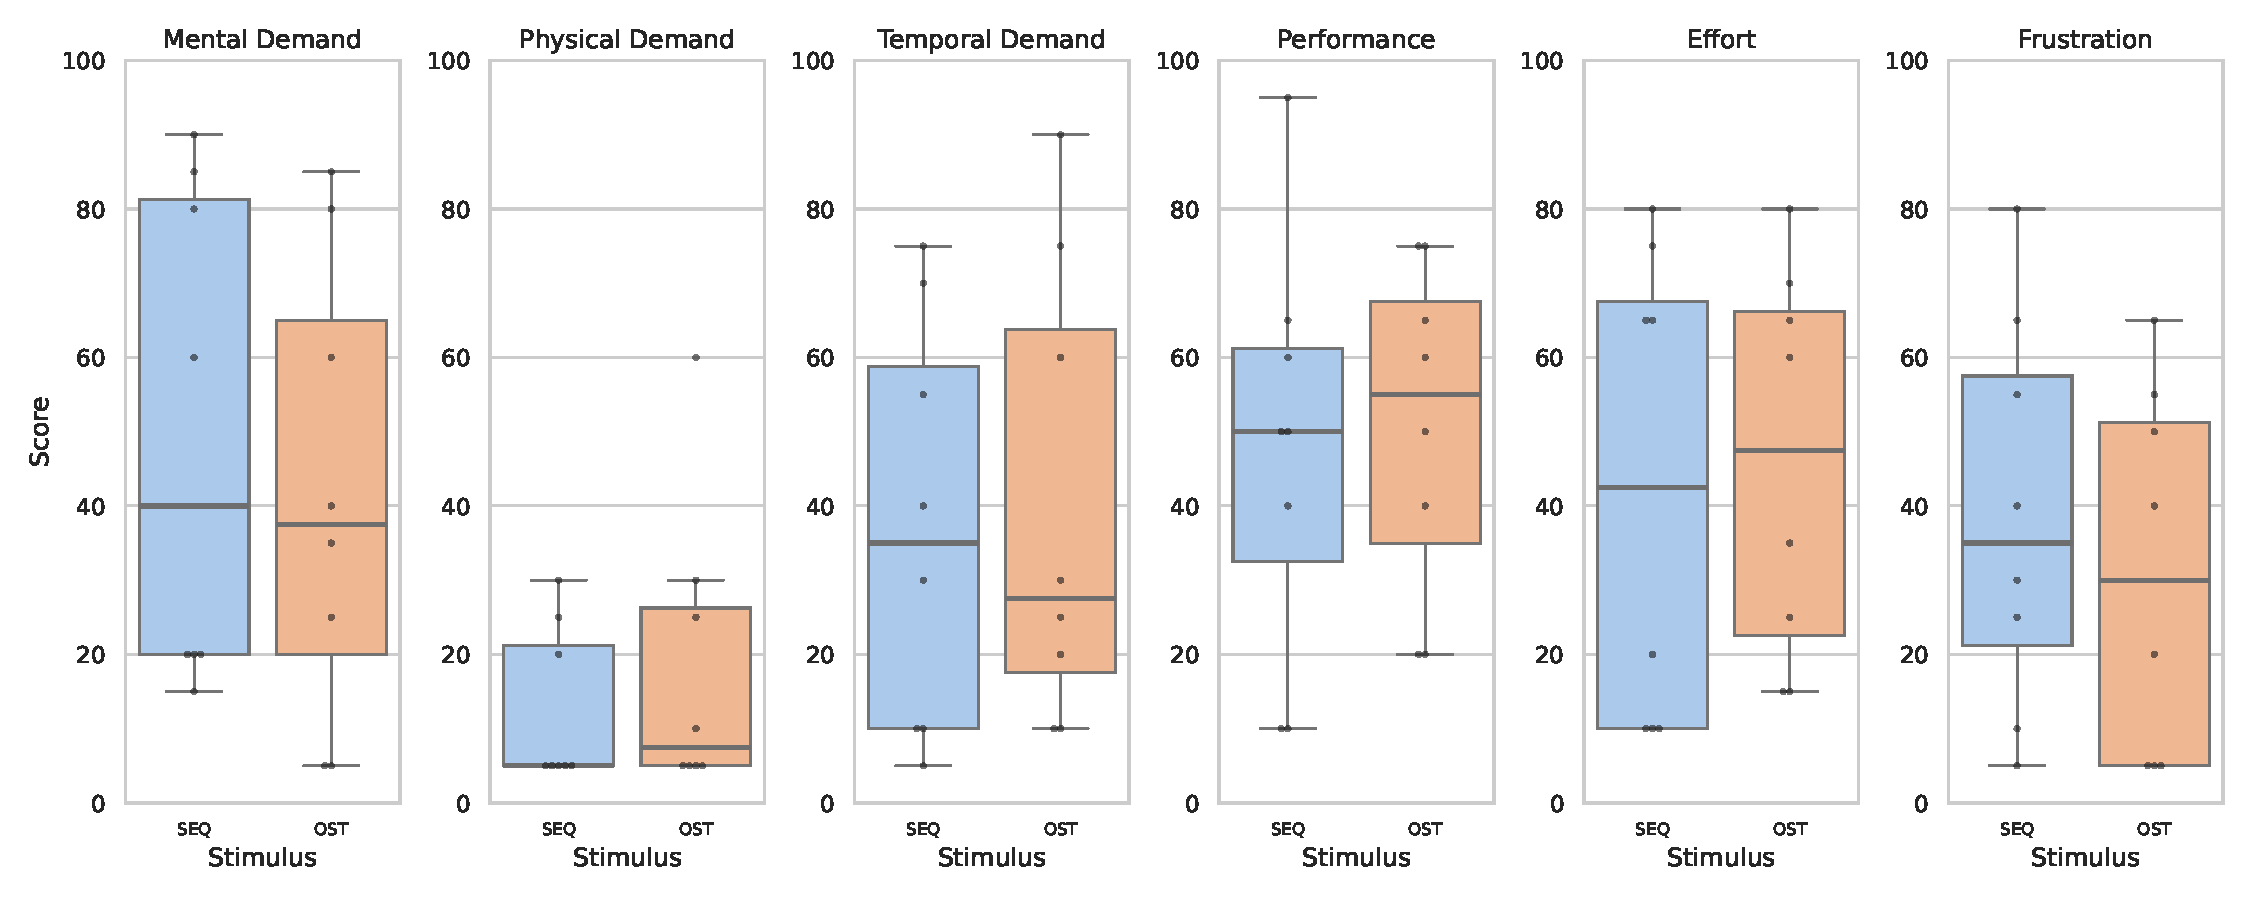
\includegraphics[width=0.5\linewidth]{src/pictures/Study2Data_questionnaire/NasaTLX.pdf}
    \caption{Nasa TLX results for the second study.}
    \label{fig:nasa_tlx_second_study}
\end{figure}
% After each study was conducted, we measuered the nasa tlx resulted as depicted in \autoref{fig:nasa_tlx_first_study}.
% The chart shows, that most dimensions look similar.
% Larger differences can be seen in \enquote{Performance} section for the outliers, as the \gls{seq} has a larger and a smaller outlier than the \gls{ost} stimulus.
% The largest median difference can be seen in the \enquote{Temporal Demand} dimension with a median of  35 for \gls{seq} and about 27 for \gls{ost}.
% The largest q2-q3 difference can be seen for the dimension \enquote{Frustration}, where the seq q1-q3 range was from about 22 to 57.5 an the \gls{ost} one from 0 to 50.

% After checking their significance using a Wilcoxon test, it shows an approaching significance in the \enquote{frustration} dimension with a p-value of $0.0656$ and a large cohens d of 0.6644,
% that shows that \gls{seq} is more frustrating for the participants than \gls{ost}.
After completing the second study, we measured participants' perceived workload using the NASA-TLX questionnaire, as shown in \autoref{fig:nasa_tlx_first_study}. 

Overall, most dimensions appear similar across conditions. However, notable differences were observed in the \enquote{Performance} category, particularly in the outliers: the \gls{seq} condition had both a higher and lower outlier compared to the \gls{ost} condition. The largest difference in medians was found in the \enquote{Temporal Demand} dimension, with \gls{seq} showing a median of $35$, compared to approximately $27$ for \gls{ost}. 

A pronounced difference in interquartile range was also visible in the \enquote{Frustration} dimension. For \gls{seq}, the IQR spanned from approximately $22$ to $57.5$, whereas for \gls{ost}, it ranged from $0$ to $50$.

Statistical analysis using a Wilcoxon signed-rank test indicated an approaching significance in the \enquote{Frustration} dimension, with a $p$-value of $0.0656$ and a large Cohen’s $d$ effect size of $0.6644$. This suggests that participants experienced more frustration under the \gls{seq} condition compared to \gls{ost}.


\begin{table}[ht]
\resizebox{\columnwidth}{!}{
\centering
\begin{tabular}{|l|l|l|l|l|}
\hline
\textbf{Question}        & \textbf{Wilcoxon test}& \textbf{p-value}       & \textbf{Significance}           &\textbf{Cohens D}\\ \hline
\textbf{Mental Demand}    & 7.5& 0.2676& Not Significant                 &0.4233\\ \hline
\textbf{Physical Demand}  & 0.0& 0.1025& Not Significant                 &-0.4656\\ \hline
\textbf{Temporal Demand}  & 9.5& 0.4444& Not Significant                 &-0.2212\\ \hline
\textbf{Performance}      & 9.0& 0.7525& Not Significant                 &-0.0925\\ \hline
\textbf{Effort}           & 7.0& 0.2274& Not Significant                 &-0.3428\\ \hline
\textbf{Frustration}      & 0.0& 0.0656& approaching
\textbf{Significant}&0.6644\\ \hline
\end{tabular}}
\caption{Results of the Friedman significance tests for the different NasaTLX dimensions with a Kendall's W Effect Size.}
\label{table:nasaTLX_significance_secondStudy_nonParam}
\end{table}


\begin{figure}
    \centering
    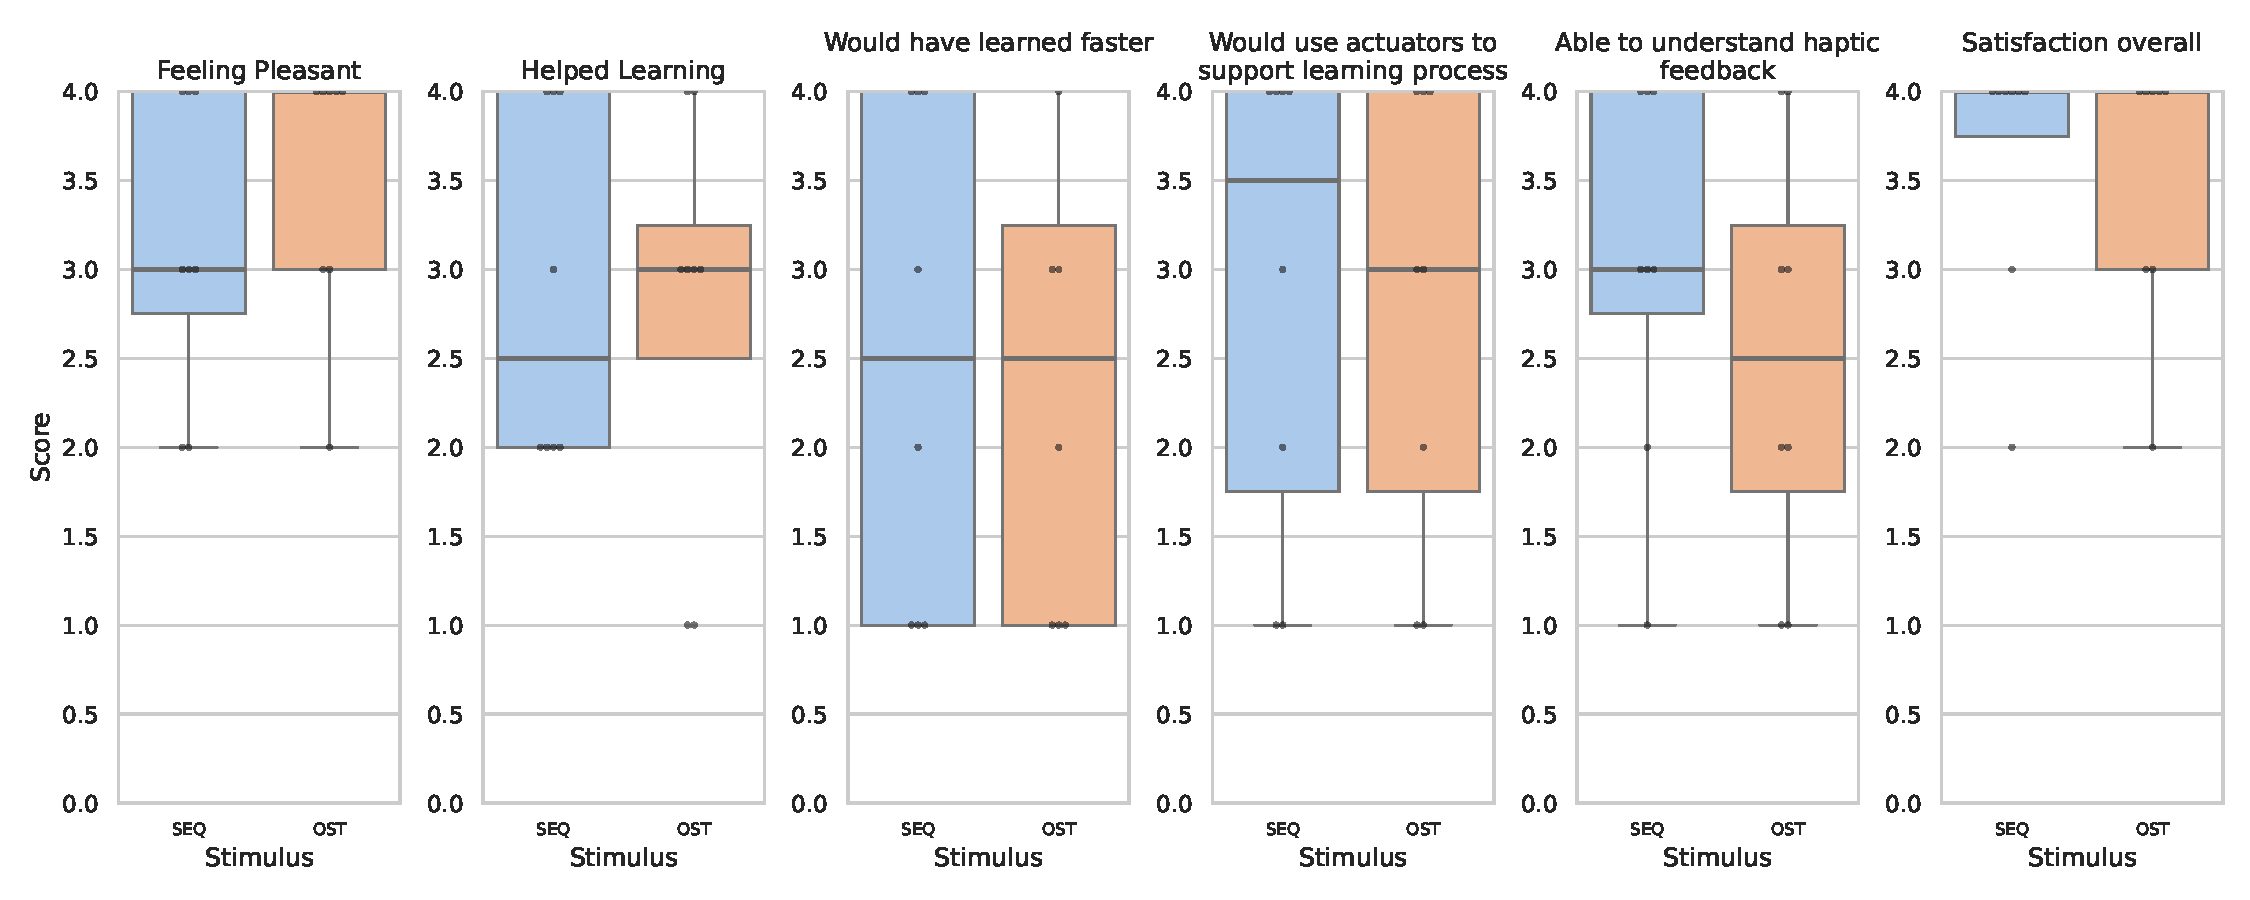
\includegraphics[width=0.5\linewidth]{src/pictures/Study2Data_questionnaire/self_evaluation.pdf}
    \caption{Usability questions results for the second study.}
    \label{fig:special_study_second_study}
\end{figure}
% After learning a word with a stimuli, we also tested for the usability for six dimensions, whose results are depicted in \autoref{fig:special_study_first_study}.
% Here the largest differences can be seen in the dimensions \enquote{Feeling Pleasant} with a large median difference of 3 for \gls{seq} and 4 for \gls{ost}.

% For \enquote{helped learning}, there is a larger difference between the q1,q3 quantile ranges, with 2 to 4 for \gls{seq} and 2.5 to 3.25 for \gls{ost}, also their medians differ with 2.5 for \gls{seq} and 3 for \gls{ost}.
% Moreover, \gls{ost} had two outliers at 1, with was not the case for \gls{seq}.
% Other median differences of 1 can be seen for the dimensions \enquote{Would use actuators to support the learning process} and \enquote{able to understand haptic feedback}, where the \gls{seq} median was better of about 1 for both of them, with 3.5 vs 3 and 2.5 to 3 for both dimensions respectively

% After testing for signifiant difference, we didn't find any as depcited in \autoref{table:individualQuestions_significance_secondStudy}.
% However, it is also depicted, that there is a approaching signifficance for the feeling pleaseant dimension with a p-value of 0.0833 and a large cohens d of -0.7246, that shows that the \gls{ost} was perceived as better for learning by the participants.
After participants learned a word using each stimulus, we evaluated usability across six dimensions. The results are shown in \autoref{fig:special_study_first_study}.

The most prominent difference was observed in the \enquote{Feeling Pleasant} dimension, where the median was notably higher for \gls{ost} at $4$, compared to $3$ for \gls{seq}. 

In the \enquote{Helped Learning} dimension, the interquartile ranges differed: $2$ to $4$ for \gls{seq}, and $2.5$ to $3.25$ for \gls{ost}, with respective medians of $2.5$ and $3.0$. Additionally, two outliers at the lowest rating (1) were recorded for \gls{ost}, which were not present in \gls{seq}. 

Other notable median differences of $1$ point were found in the dimensions \enquote{Would use actuators to support the learning process} and \enquote{Able to understand haptic feedback}, where \gls{seq} had higher median scores—$3.5$ vs.\ $3.0$ and $3.0$ vs.\ $2.0$, respectively.

Statistical testing did not reveal any significant differences across the dimensions, as shown in \autoref{table:individualQuestions_significance_secondStudy}. However, an approaching significance was observed in the \enquote{Feeling Pleasant} dimension, with a $p$-value of $0.0833$ and a large Cohen's $d$ of $-0.7246$, suggesting that \gls{ost} was perceived as more pleasant and potentially more effective for learning by the participants.



\begin{table}[ht]
\resizebox{\columnwidth}{!}{
\centering
\begin{tabular}{|l|l|l|l|l|}
\hline
\textbf{Question}                              & \textbf{Wilcoxon test}& \textbf{p-value}       & \textbf{Significance}           &\textbf{Cohens D}\\ \hline
\textbf{Feeling Pleasant}                      & 0.0& 0.0833& approaching
\textbf{Significant}&-0.7246\\ \hline
\textbf{Helped Learning}                       & 6.0& 0.6547& Not Significant                 &0.1498\\ \hline
\textbf{Would have learned faster}             & 5.0& 0.4795& Not Significant                 &0.0\\ \hline
\textbf{Would use actuators to support learning process} & 4.0& 0.7055& Not Significant                 &0.1261\\ \hline
\textbf{Able to understand haptic feedback}    & 5.5& 0.2795& Not Significant                 &0.2958\\ \hline
\textbf{Satisfaction overall}& 2.0& 0.5637& Not Significant                 &0.1950\\ \hline
\end{tabular}}
\caption{Results of the Wilcoxon significance tests for the different self-assessment dimensions with a Cohens D Effect Size.}
\label{table:individualQuestions_significance_secondStudy}
\end{table}



\begin{figure}
    \centering
    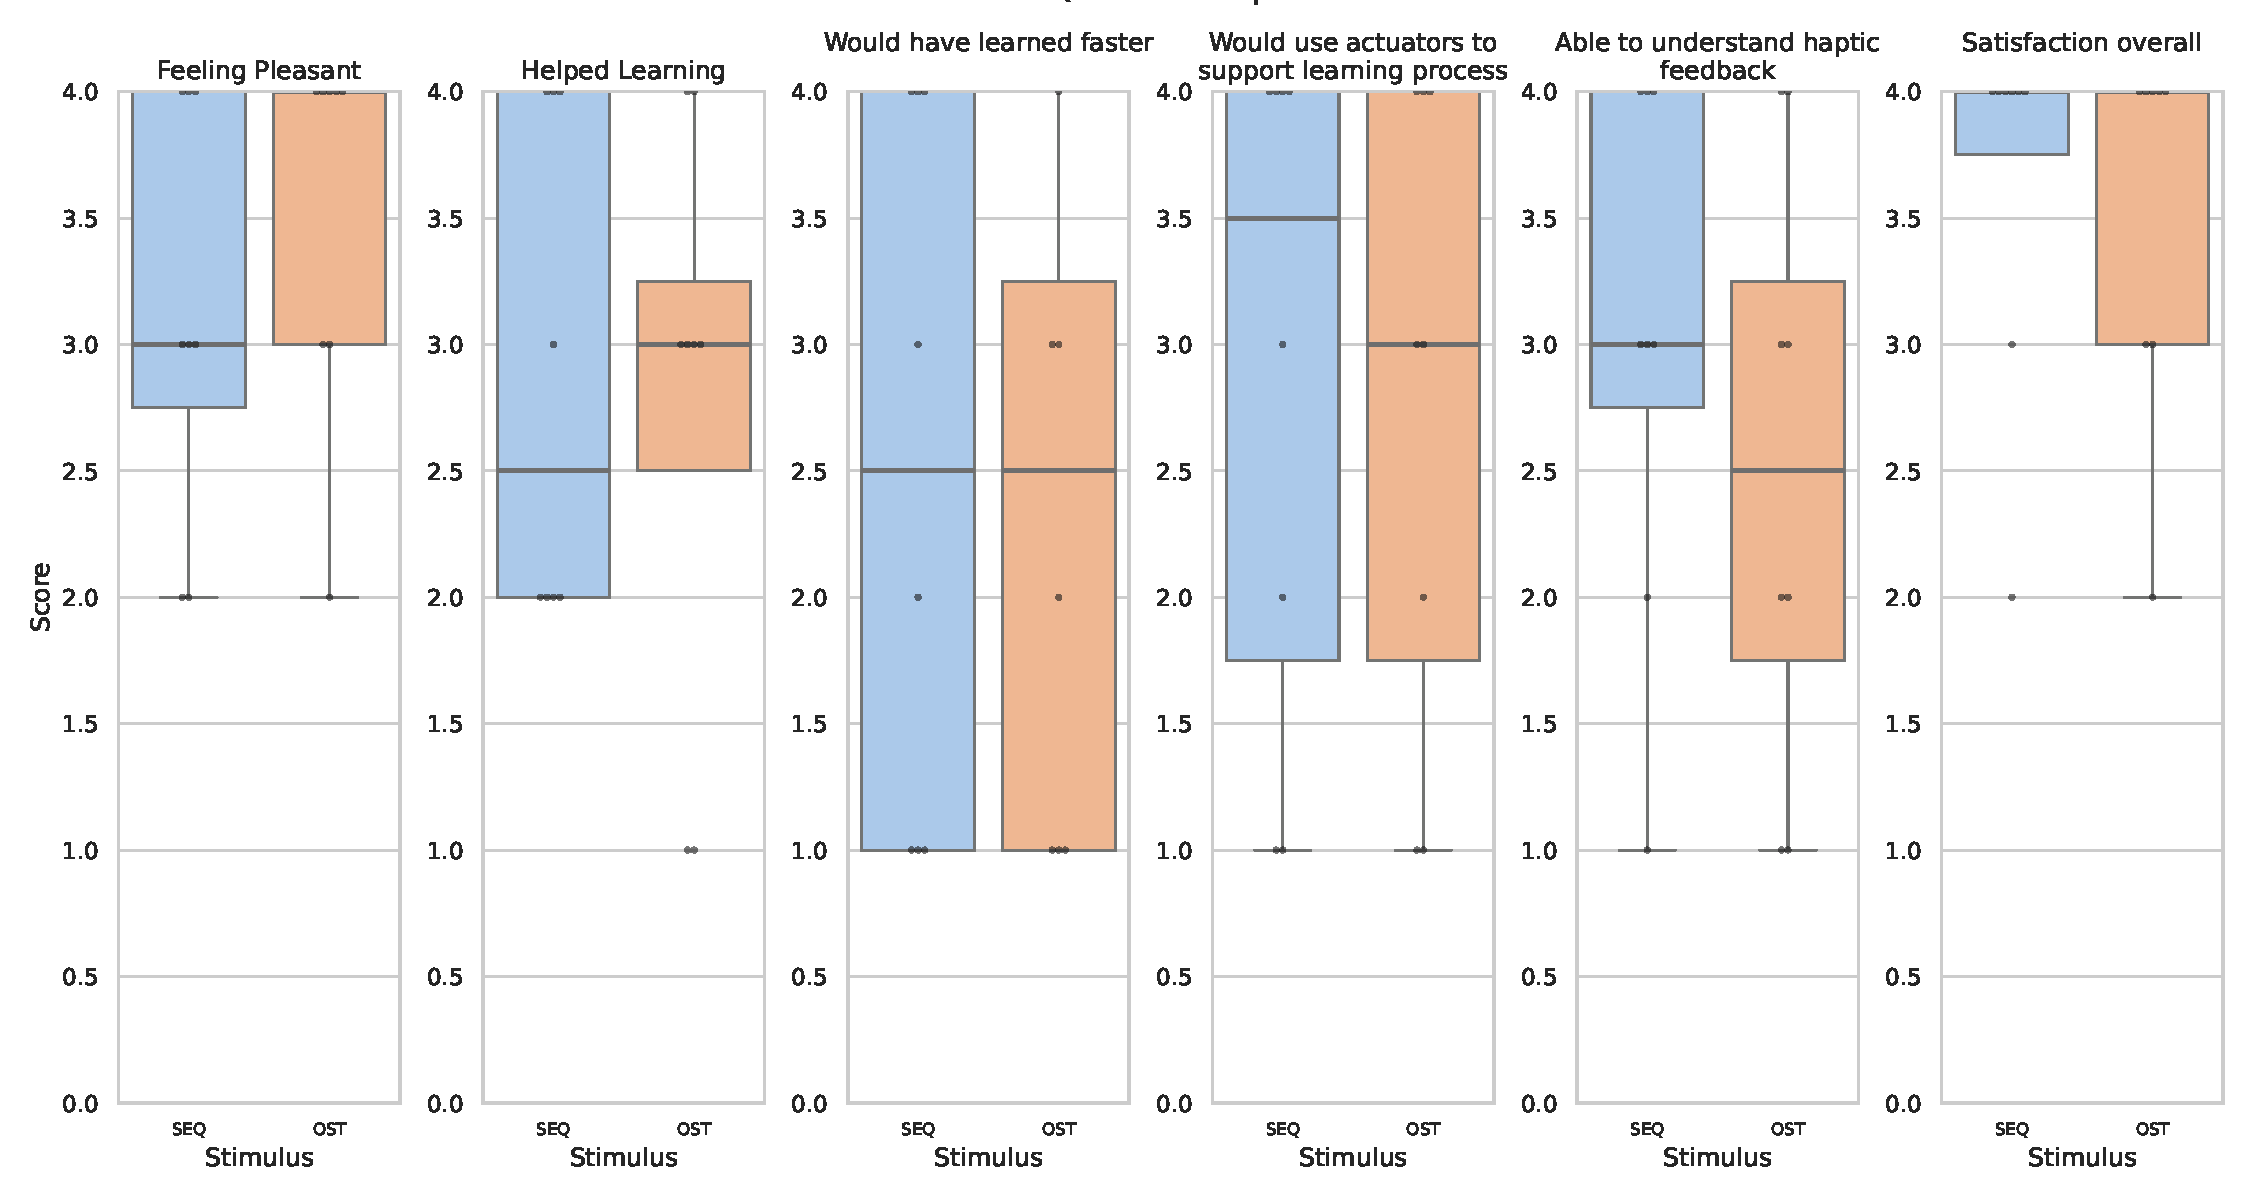
\includegraphics[width=0.5\linewidth]{src/pictures/Study2Data_questionnaire/questions_special_study2.pdf}
    \caption{Compare Results.}
    \label{fig:compare_results_second_study}
\end{figure}
% Lastly we let the participants compare each of the encodings against each other.
% The results are depicted in \autoref{fig:compare_results_second_study},  with 5/8 participants saying that \gls{seq} is the better encoding for \enquote{distinguishability} and also for \enquote{helped learning}, but only 3/8 stating that it is the \enquote{more comfortable encoding}.
% However, there is no significance in this, as measured using a $\chi^2$ test, with p-values of 0.4795, as depicted in \autoref{table:individualQuestions_significance_secondStudy}.
Lastly, participants were asked to directly compare the two encoding methods. The results are shown in \autoref{fig:compare_results_second_study}. 

A majority of participants (5 out of 8) preferred \gls{seq} over \gls{ost} for both \enquote{Distinguishability} and \enquote{Helped Learning}. However, only 3 out of 8 participants found \gls{seq} to be the \enquote{More Comfortable Encoding}.

A $\chi^2$ test was conducted to assess the significance of these preferences. The results showed no statistically significant differences, with a $p$-value of $0.4795$, as reported in \autoref{table:individualQuestions_significance_secondStudy}.


\begin{table}[ht]
\resizebox{\columnwidth}{!}{
\centering
\begin{tabular}{|l|l|l|l|}
\hline
\textbf{Question}                              & \textbf{$\chi^2$ test}& \textbf{p-value}       & \textbf{Significance}           \\ \hline
\textbf{Better distinguishable encoding}& 0.5& 0.4795& Not Significant                 \\ \hline
\textbf{Helped Learning encoding}& 0.5& 0.4795& Not Significant                 \\\hline
 \textbf{Most comfortable encoding}& 0.5& 0.4795& Not Significant                 \\\hline
\end{tabular}}
\caption{Results of the Wilcoxon significance tests for the different self-assessment dimensions with a Cohens D Effect Size.}
\label{table:individualQuestions_significance_secondStudy}
\end{table}
